\chapter{An Issue of Trust}
\label{chap:trust}

Trust and privacy are closely related qualities in
computing~\cite{flowerday2006}. Can we maintain our digital privacy
without having to trust anyone? We can imagine scenarios that maintain
privacy without trust, but they generally involve only storing data on
self-designed, built, and programmed devices that never leave our
possession. Such arrangements are, at best, impractical for the vast
majority of users, and at worst, simply not possible to achieve
today. The range of manufactures, suppliers, and service providers
inherent in the modern computing landscape require that we make
decisions regarding whom to trust at every step of any digital
interaction in which we partake.

The cloud computing model, by its very nature, further amplifies the
number of parties we must trust. But what does it mean to trust a
third party in the cloud? Before discussing the details of an SSaaS
ecosystem, it's helpful to further define ``trust''. In this chapter,
I define a model for analyzing trust and apply this model to compare
various traditional software and technology deployments to SSaaS-backed
options.

\section{Analyses Framework}
\label{chap:trust:framework}

Generally, when we use modern computing devices and services, we must
trust third-party manufactures and service providers with our
data. The manner in which this third party trust relates to the
privacy of user data has two main factors: how much trust do we place
in third parties (e.g. how much of our personal data do we grant them
access to), and in what manner can they violate this trust (e.g. how
can they abuse the access they are granted). I will thus evaluate
computing trust models across two main axes: the \emph{degree} of
trust we must place in third parties, and the manner in which this
trust might be \emph{violated}. Our ideal trust model for a given use
case will minimize the degree of third party trust while also
minimizing the likelihood that such trust will be violated.

In terms of degrees of trust, we can entrust third parties with the
following data-related capabilities:

\begin{packed_desc}
\item[Storage (S):] \hfill \\
  Can a third party faithfully store private user data and make it
  available to the user upon request? Misuse of this capability may
  result in a loss of user data, but won't generally result in the
  exposure of user data.
\item[Access (R):] \hfill \\
  Can a third party read and interpret the private user data they
  store? Misuse of this capability may result in the exposure of user
  data.
\item[Manipulation (W):] \hfill \\ Can a third party modify the
  private user data to which they have access? Misuse of this
  capability may result in the ability to manipulate a user
  (e.g. changing appointments on a user's calendar, etc).
\item[Meta-analysis (M):] \hfill \\
  Can a third party gather user metadata related to any stored private
  user data? Misuse of this capability may result in the ability to
  infer private user data (e.g. who a user is friends with based on
  data sharing patterns).
\end{packed_desc}

I'll define a trust violation as occurring when a third party
exercises any of the above capabilities without explicit user
knowledge and permission. Put another way, a trust violation occurs
whenever a third party leverages a capability with which they are
entrusted in a manner in which the user does not expect the capability
to be leveraged.

I define several types of trust violations based on the manner in
which the violation occurs and the motivations behind it:

\begin{packed_desc}
\item[Implicit (P):] \hfill \\
  This class of trust violation occurs when a third party violates a
  user's trust in a manner approved by the third party. An example
  might be sharing user data with a business partner (e.g. an
  advertiser). Often these forms of violations aren't really
  ``violations'' in the sense that a user may have clicked though a
  Terms of Service agreement that granted implicit permission for such
  use, but if the third party is engaging in behavior that the user
  would not generally expect, an implicit trust violation has
  occurred.
\item[Compelled (C):] \hfill \\
  This class of trust violation occurs when a third party is compelled
  by another actor to violate a user's trust. The most common example
  would be a third party being forced to turn over user data or
  records in response to a request from the government with
  jurisdiction over the party.
\item[Unintentional (U):] \hfill \\
  This form of violation occurs when a third party unintentionally
  discloses or manipulates user data. An example would be a coding
  error that allows either the loss of or unfettered access to user
  data.
\item[Insider (I):] \hfill \\
  This class of violation occurs when a privileged adversary within
  the third party violates a user's trust without the permission or
  knowledge of the third party. An example would be a cloud service
  provider employee accessing or disclosing private user data without
  authorization.
\item[Outsider (O):] \hfill \\
  This class of violation occurs when an external adversary gains
  unauthorized access to private user data stored by third party. An
  example would be an adversary exploiting a bug in a third party's
  authorization infrastructure to gain unauthorized access to user
  data.
\end{packed_desc}

\section{Traditional Model}
\label{chap:trust:traditional}

\begin{figure}[t]
  \centering
  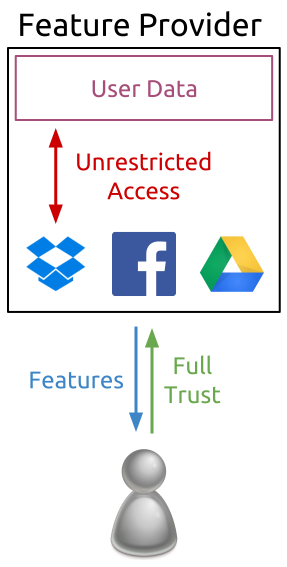
\includegraphics[height=175px]{./figs/out/TrustModel-Traditional.pdf}
  \caption{Traditional Trust Model}
  \label{fig:trust-traditional}
\end{figure}

Existing cloud services are not generally well optimized for
maximizing user privacy. Such services tend to apply an all-or-nothing
trust model where a user must seed a high degree of trust to each
service in order to reap the benefits each service provides. Figure
\ref{fig:trust-traditional} shows the basic trust-for-features
relationship between a user, their private data, and a traditional
cloud service provider.

We can analyze the Dropbox example from \S~\ref{chap:intro:example}
using my proposed framework. To begin, what capabilities is a normal
Dropbox user entrusting to Dropbox? Clearly, users must trust Dropbox
to faithfully store their data since that is Dropbox's core purpose,
so we have granted Dropbox the \emph{S} capability. Furthermore users
must also grant Dropbox the ability to read and access their data
(i.e. the \emph{R} capability) in order to support Dropbox's sharing
and syncing features. While Dropbox doesn't generally utilize it,
users are also effectively granting the manipulation (\emph{W})
capability as well since the user has no mechanisms for ensuring that
Dropbox can't manipulate their data. Finally, Dropbox has full access
to user metadata related to their usage of the service, granting them
the \emph{M} capability. Thus, Dropbox users must trust Dropbox with
all possible capabilities.

But how likely is it that Dropbox might misuse any of these
capabilities, thus violating the user's trust and privacy? In terms of
implicit violations (\emph{I}), Dropbox charges users for storage, and
thus shouldn't generally rely on reading or sharing user data for
advertising purposes. Furthermore, such a business model relies on
Dropbox remaining in its paying users' good graces, disincentivizing
potentially questionable behavior. None the less, there is evidence of
Dropbox opening user files for unknown
reasons~\cite{vintsurf-dropbox}, which might indicate a possible
\emph{I} violation. The user has no way to prevent an \emph{I}
violation when using Dropbox, so we can do no more than give Dropbox
the benefit of the doubt in this area.

In terms of compelled (\emph{C}) violations, Dropbox is a US-based
company, and is thus susceptible to a variety of government-sponsored
data requested, from subpoenas issued under the Third Party
Doctrine~\cite{thompson-thirdparty}, to probable cause search
warrants~\cite{us-constitution-amend4}, to National Security
Letters~\cite{fbi-nsl}, to FISC~\cite{fisc} orders. Dropbox publishes
a transparency report~\cite{dropbox-transparency} indicating how
frequently they are compelled to violate user privacy. Recent versions
of this report indicate that Dropbox receives a few hundred requests
for various user data every 6 months.

Unintentional (\emph{U}), Insider (\emph{I}), or Outsider (\emph{O})
violations are all possibilities when using Dropbox. On the \emph{U}
front, Dropbox had an incident in 2011 that allowed anyone to log into
the service using any password for a 5 hour
period~\cite{dropbox-authbug}. Thus far, Dropbox appears to have
avoided any \emph{I}-type violations, but it has been the target of
various \emph{O}-type attempted violations, primarily built around
advisories who obtain common user
passwords~\cite{dropbox-passwords}. Needless to say, while Dropbox
works to avoid these kinds of violations, they are certainly still
possible, have occurred in the past, and may well occur in the future.

As we can see, a traditional cloud service like Dropbox currently
requires an essentially full degree of user trust (i.e. \emph{S},
\emph{R}, \emph{W}, and \emph{M} capabilities) while also being
susceptible to a full range of trust violations (e.g. \emph{P},
\emph{C}, \emph{U}, \emph{I}, and \emph{O} type violations). Dropbox
is not unique. Other modern computing services from social media
sites, to file lockers, to communication systems all suffer from the
same high-trust, high potential for violations paradigm.

\section{SSaaS Model}
\label{chap:trust:ssaas}

\begin{figure}[t]
  \centering
  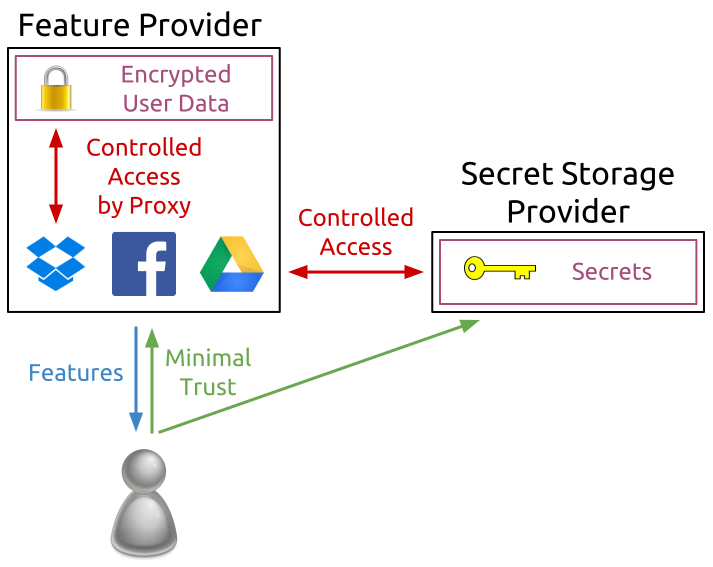
\includegraphics[height=175px]{./figs/out/TrustModel-Seperated.pdf}
  \caption{SSaaS Trust Model}
  \label{fig:trust-ssaas}
\end{figure}

In order to enhance user privacy in the cloud, we must move beyond the
traditional full-trust, easily violated model presented in
\S~\ref{chap:trust:traditional}. Of the two components of my trust
framework, degree of trust and potential for violation, degree is the
easier to control quality: what capabilities to trust a cloud provider
with is largely within the user's control, where as the method in
which trust might be violated is largely outside of a user's
control. I will thus focus my solution on mitigating degree of trust
first while disincentivizing methods of violation second.

The ideal trust model begins with the principle of least
privilege~\cite{saltzer1975}: we should only afford a cloud provider
the minimal degree of trust necessary to provide the intended
features. Furthermore, in order to monitor cloud providers for
potential trust violations, we would also like to maintain some degree
of auditing over any capability we entrust to a provider. Minimal,
audited trust is the basis of my ideal trust model.

Applying this ideal trust model to the previous Dropbox example, I
conclude that Dropbox should really only be afforded the storage
(\emph{S}) capability: after all, there is no real need for Dropbox to
ever be able to access (\emph{R}) or manipulate (\emph{W}) user data
in order to blindly sync files across device or share them with other
users. While Dropbox does not need the metadata (\emph{M}) capability
to simply support the desired user case, it is far more difficult for
the user to limit this capability then the \emph{R} or \emph{W}
capabilities. I thus will also concede this capability to Dropbox as
well. We have thus reduced Dropbox's capabilities from four (full
trust) to two (minimal trust).

But how can we enforce this limited trust profile when using Dropbox?
Figure~\ref{fig:trust-ssaas} shows my proposed SSaaS solution to this
problem. I introduce a new actor: the Secret Storage Provider (SSP)
into the mix. I then restrict the user to only storing encrypted and
authenticated data with Dropbox. The user stores the associated
encryption and verification keys with the SSP. Assuming we utilize
strong encryption and integrity systems like AES~\cite{nist2001} +
CMAC~\cite{dworkin2005}, Dropbox can not feasibly decrypt and access
the user's data nor can they manipulate user data without
detection. Storing the keys with an SSP, as opposed to simply forcing
the user to maintain them manually, has a number of benefits: namely,
it affords users continued support for simple sharing and syncing use
cases. As long as the user's Dropbox client can communicate with the
SSP from any location where they can also communicate with Dropbox,
the user can continue to utilize Dropbox as they traditionally would,
but with significantly less trust in Dropbox itself.

But have we simply replaced one third party with another? Why is the
SSP any more trustworthy than Dropbox itself? There are several reason
why we might expect an SSP to be less prone to trust violations then a
feature provider like Dropbox. I'll discuss these in
\S\ref{chap:ssaas}. But in terms of degrees of trust, we really aren't
affording the SSP any greater degree of trust then Dropbox. Both are
entrusted with the \emph{S} and \emph{M} capabilities, but neither has
the \emph{R} or \emph{W} capability: Dropbox has limited capabilities
because it only holds encrypted and authenticated user data, and the
SSP has limited capabilities because it holds no direct user data at
all, only the cryptographic keys used to protect such data. As long as
the SSP faithfully guards the secret keys they store, the trust model
holds. There are a few new risks in the SSaaS model, however. If both
the feature provider (e.g. Dropbox) and the SSP are located in the
same regulatory jurisdiction, it may still be possible for a single
entity to compel (\emph{C}-type violation) them both or provide data
that would allow an adversary to elevate their capabilities to include
\emph{R} and \emph{W}. Likewise, if Dropbox and the SSP collude to
violate a user's trust, a similar capability elevation will
occur. This latter point introduces a new violation type into my
framework:

\begin{packed_desc}
\item[Colluding (L):] \hfill \\ This class of violation occurs when
  multiple partially-trusted parties collude to gain capabilities over
  user data beyond what the user intended each individually to
  have. An example would be an SSP sharing the user's encryption keys
  with the feature provider storing the corresponding encrypted data.
\end{packed_desc}

This framework provided a basis for analyzing third party trust as
well as the basic argument in favor of SSaaS as a trust-reducing
system. I discuss SSP trust and violation mitigation further in
Chapter~\ref{chap:ssaas}.

%%  LocalWords:  SSaaS FISC SSP CMAC
